% ==== DISCRIMINATING AGAINST QCD Zy PRODUCTION SECTION ====

The biggest challenge in this analysis is managing the dominant background,
\ac{QCD} \Zyjj production. Like the signal process, this background has a real Z
boson and photon. The difference is the origin of the jets, here not from a
boson decay but more likely radiated from the initial or final state.
%
Identifying and exploiting the differences in jet kinematics between this
background and the signal is therefore key to maximising the sensitivity of the
measurement. This section is dedicated to discussing this problem; the word
`signal' is used here to refer to \ac{EW} V\Zy production and `background'
refers solely to \ac{QCD} \Zyjj production.

%TODO give Feynman diagrams? Or reference previous Feynmans

% Talk about kinematic differences
There are a small number of kinematic distributions which exhibit a large
difference between signal and background that could be exploited effectively by
a cut. The dijet mass, $m_{jj}$, is an obvious example as for the signal it
peaks around the W/Z boson mass but for the background resembles a continuum.

For many more variables however, the differences are more subtle. There may be
an obvious difference in shape between signal and background
but there is no obvious cut or set of cuts that would create a signal-rich
region. Figure \ref{fig:vzy-bdt-ewvqcd} shows some distributions with the
largest signal-background discrepancies.

% m_jj and cos_theta_CS_jj show cuttable differences

\begin{figure}
  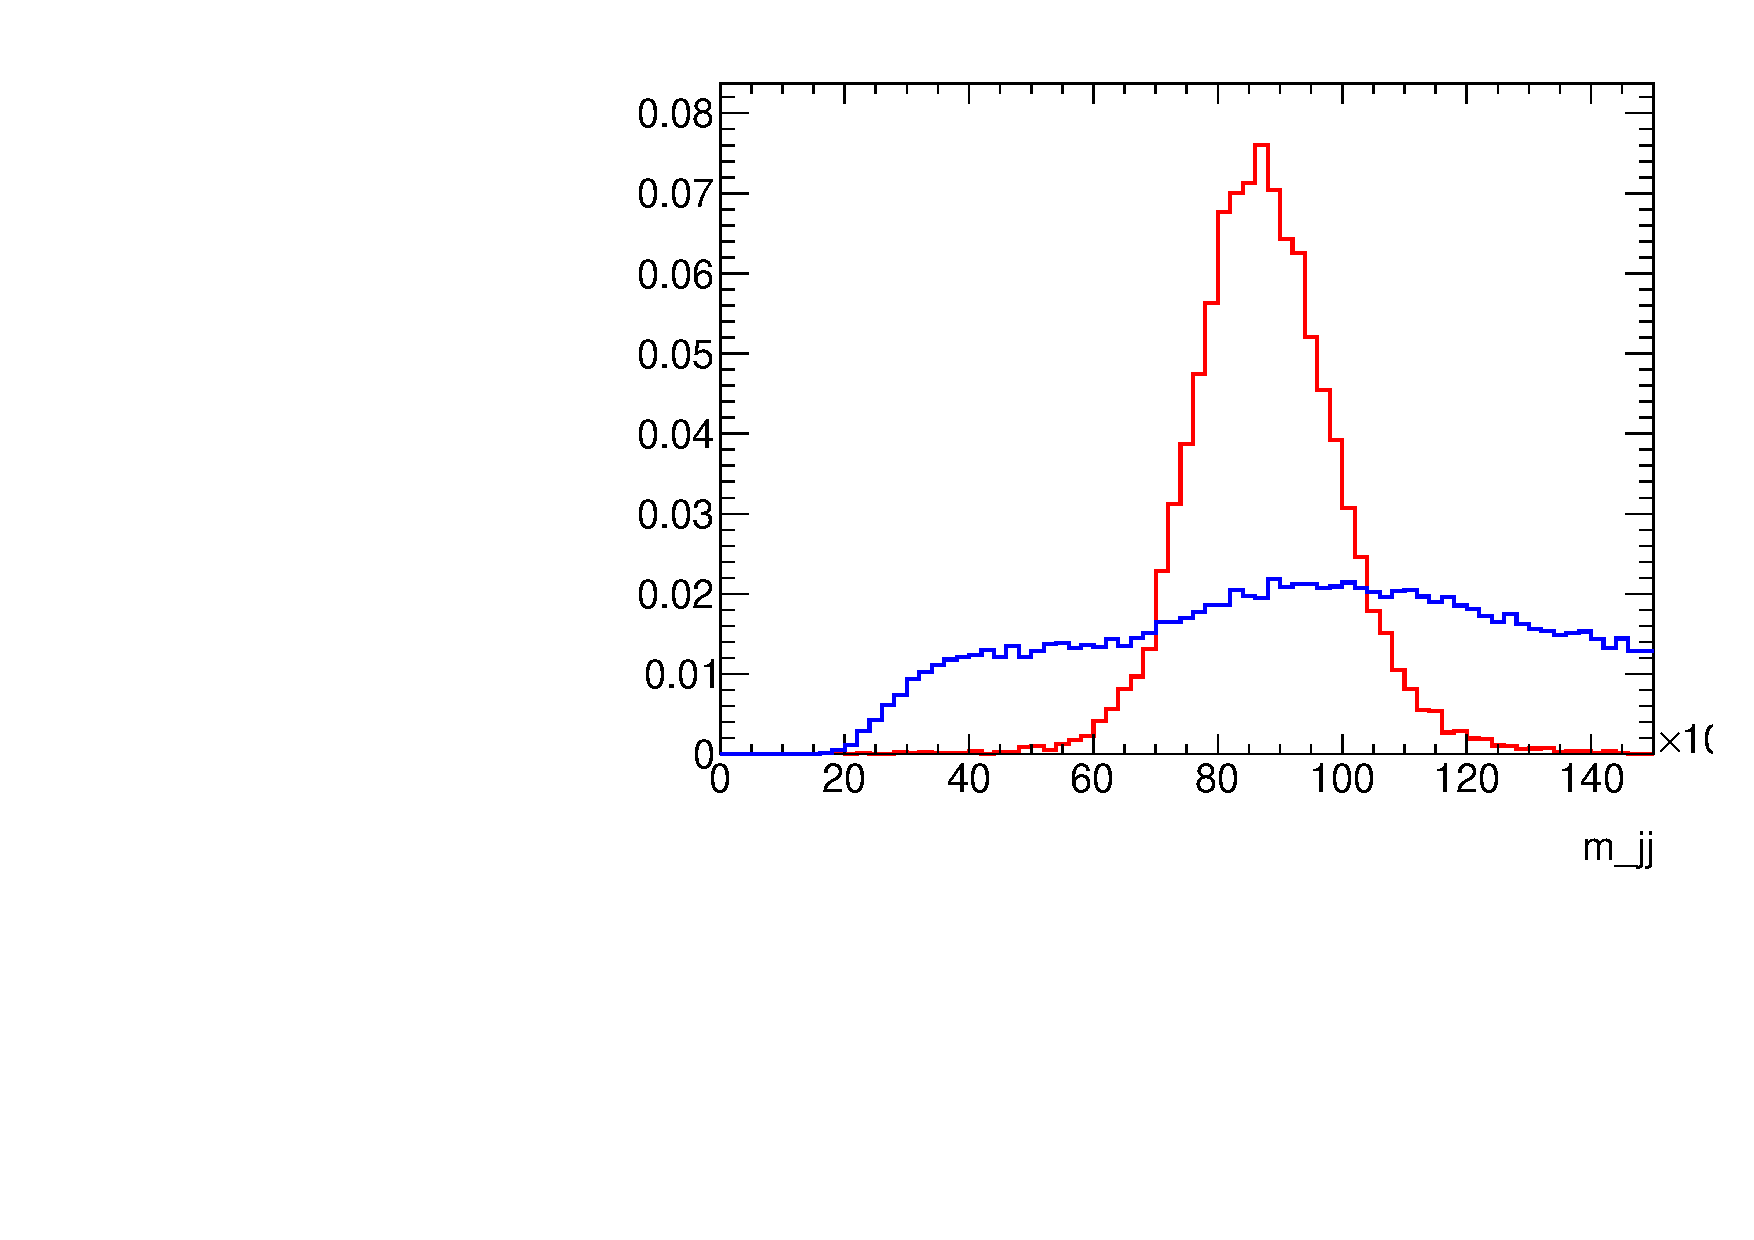
\includegraphics[width=.49\textwidth]{\resource{EWvQCD/m_jj.pdf}}
  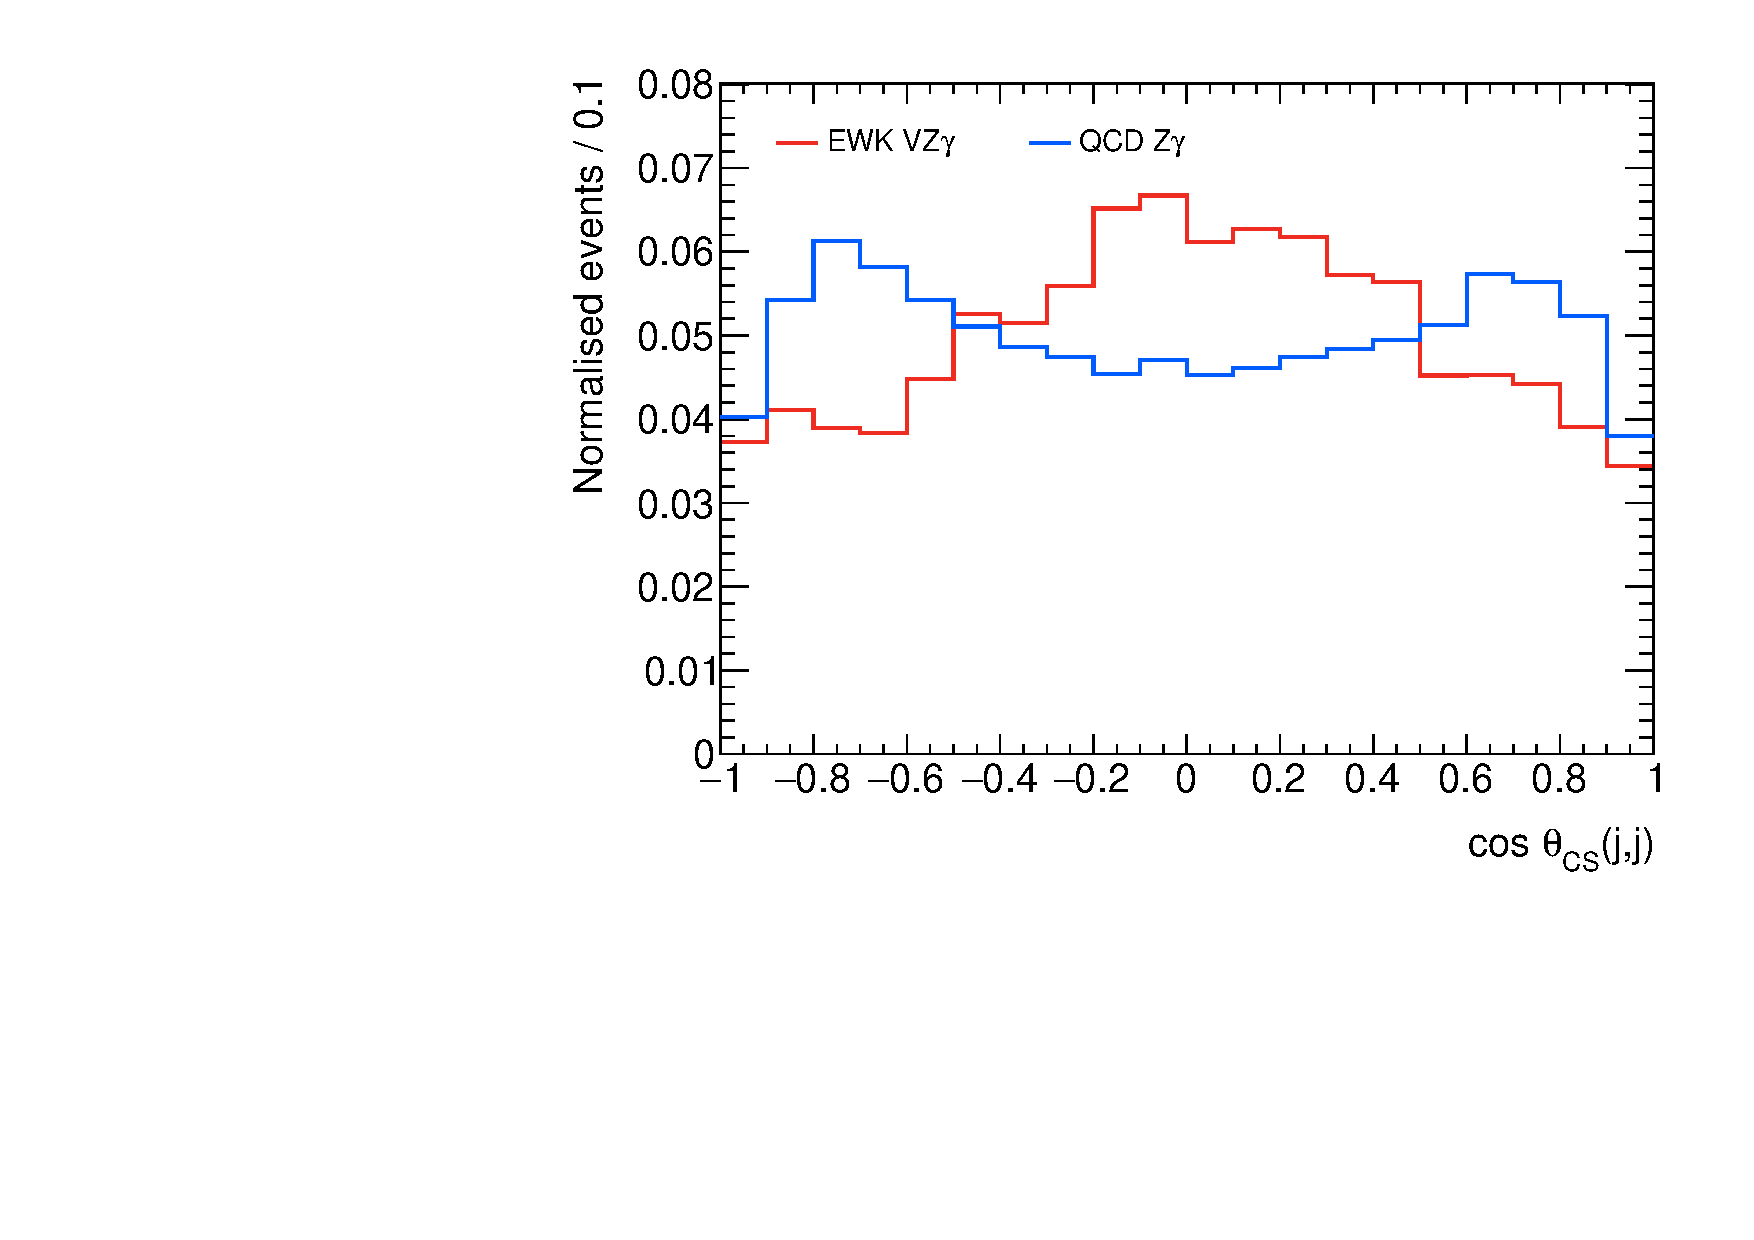
\includegraphics[width=.49\textwidth]{\resource{EWvQCD/cos_theta_CS_jj.pdf}}
  \\
  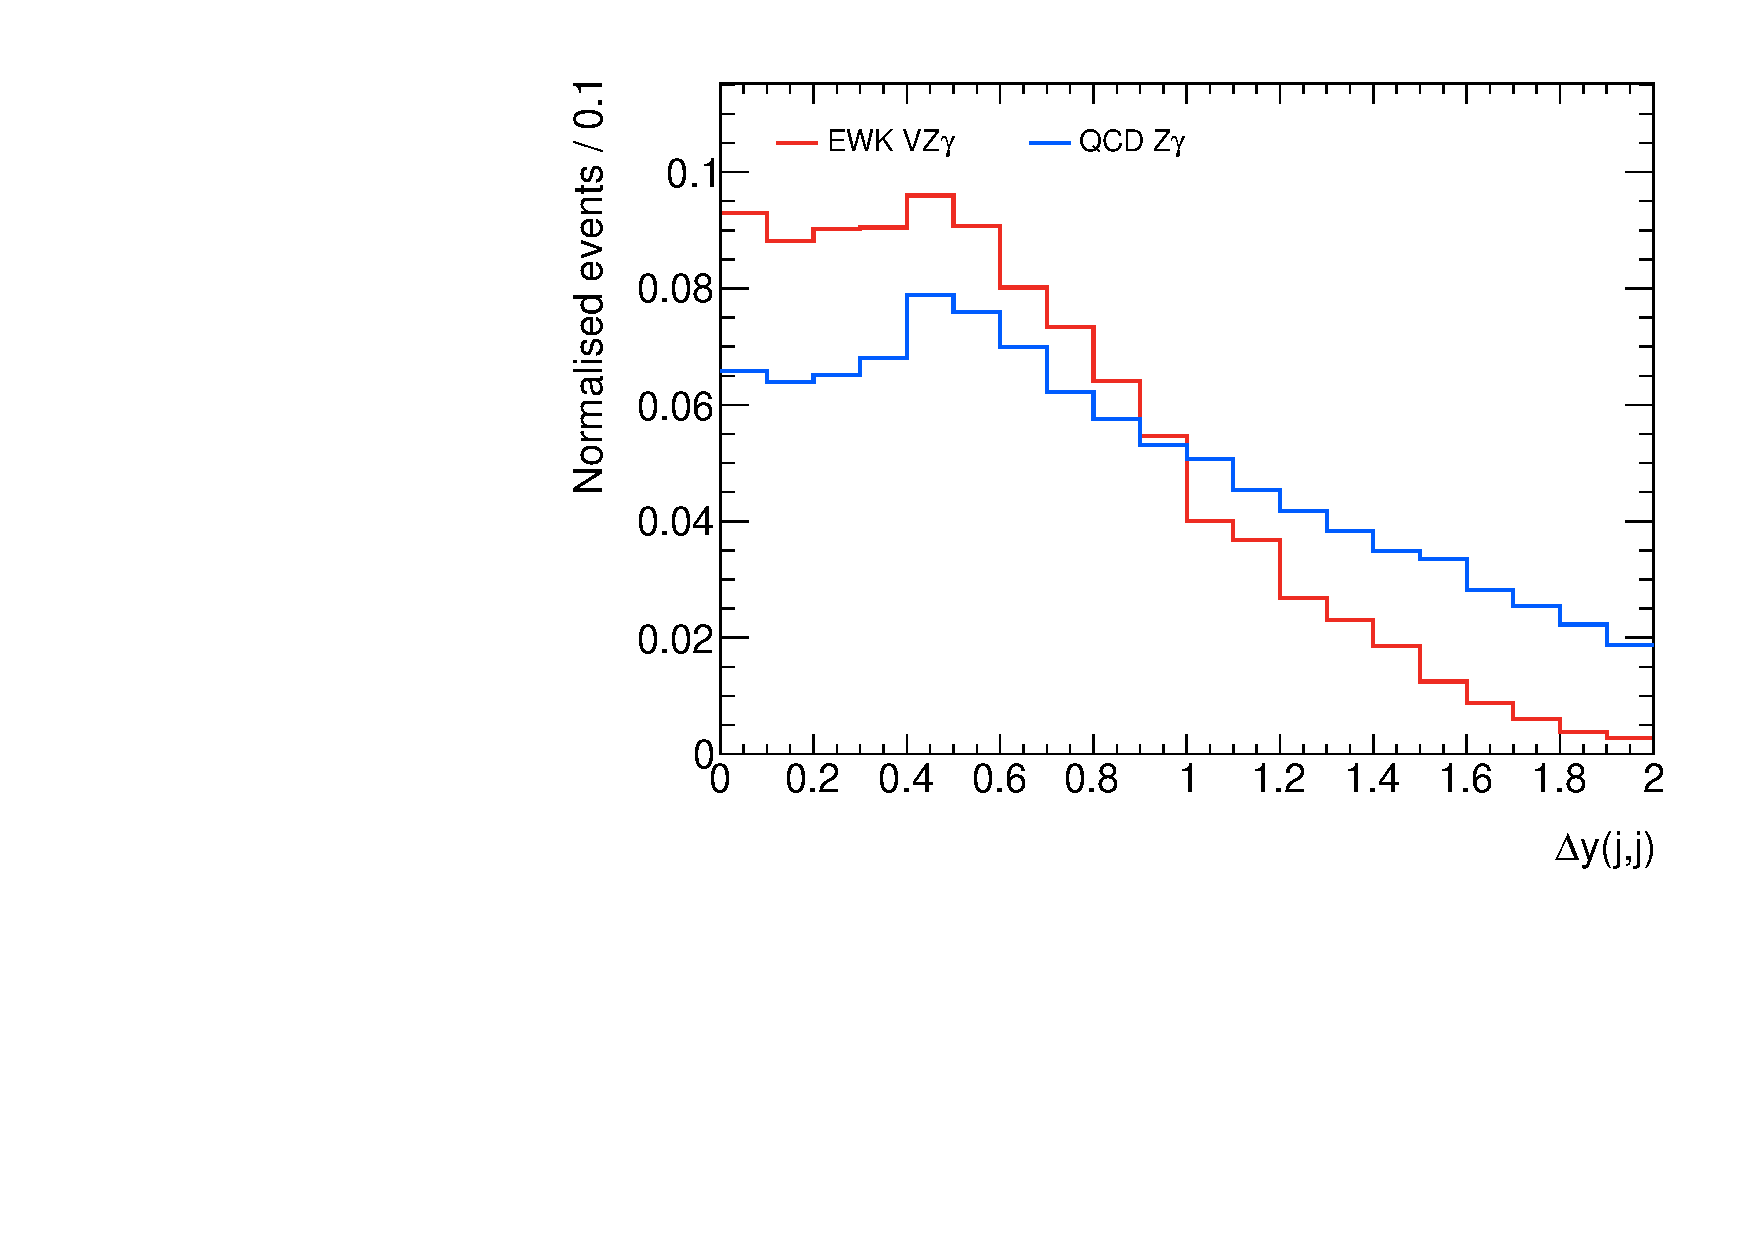
\includegraphics[width=.49\textwidth]{\resource{EWvQCD/Dy_j_j.pdf}}
  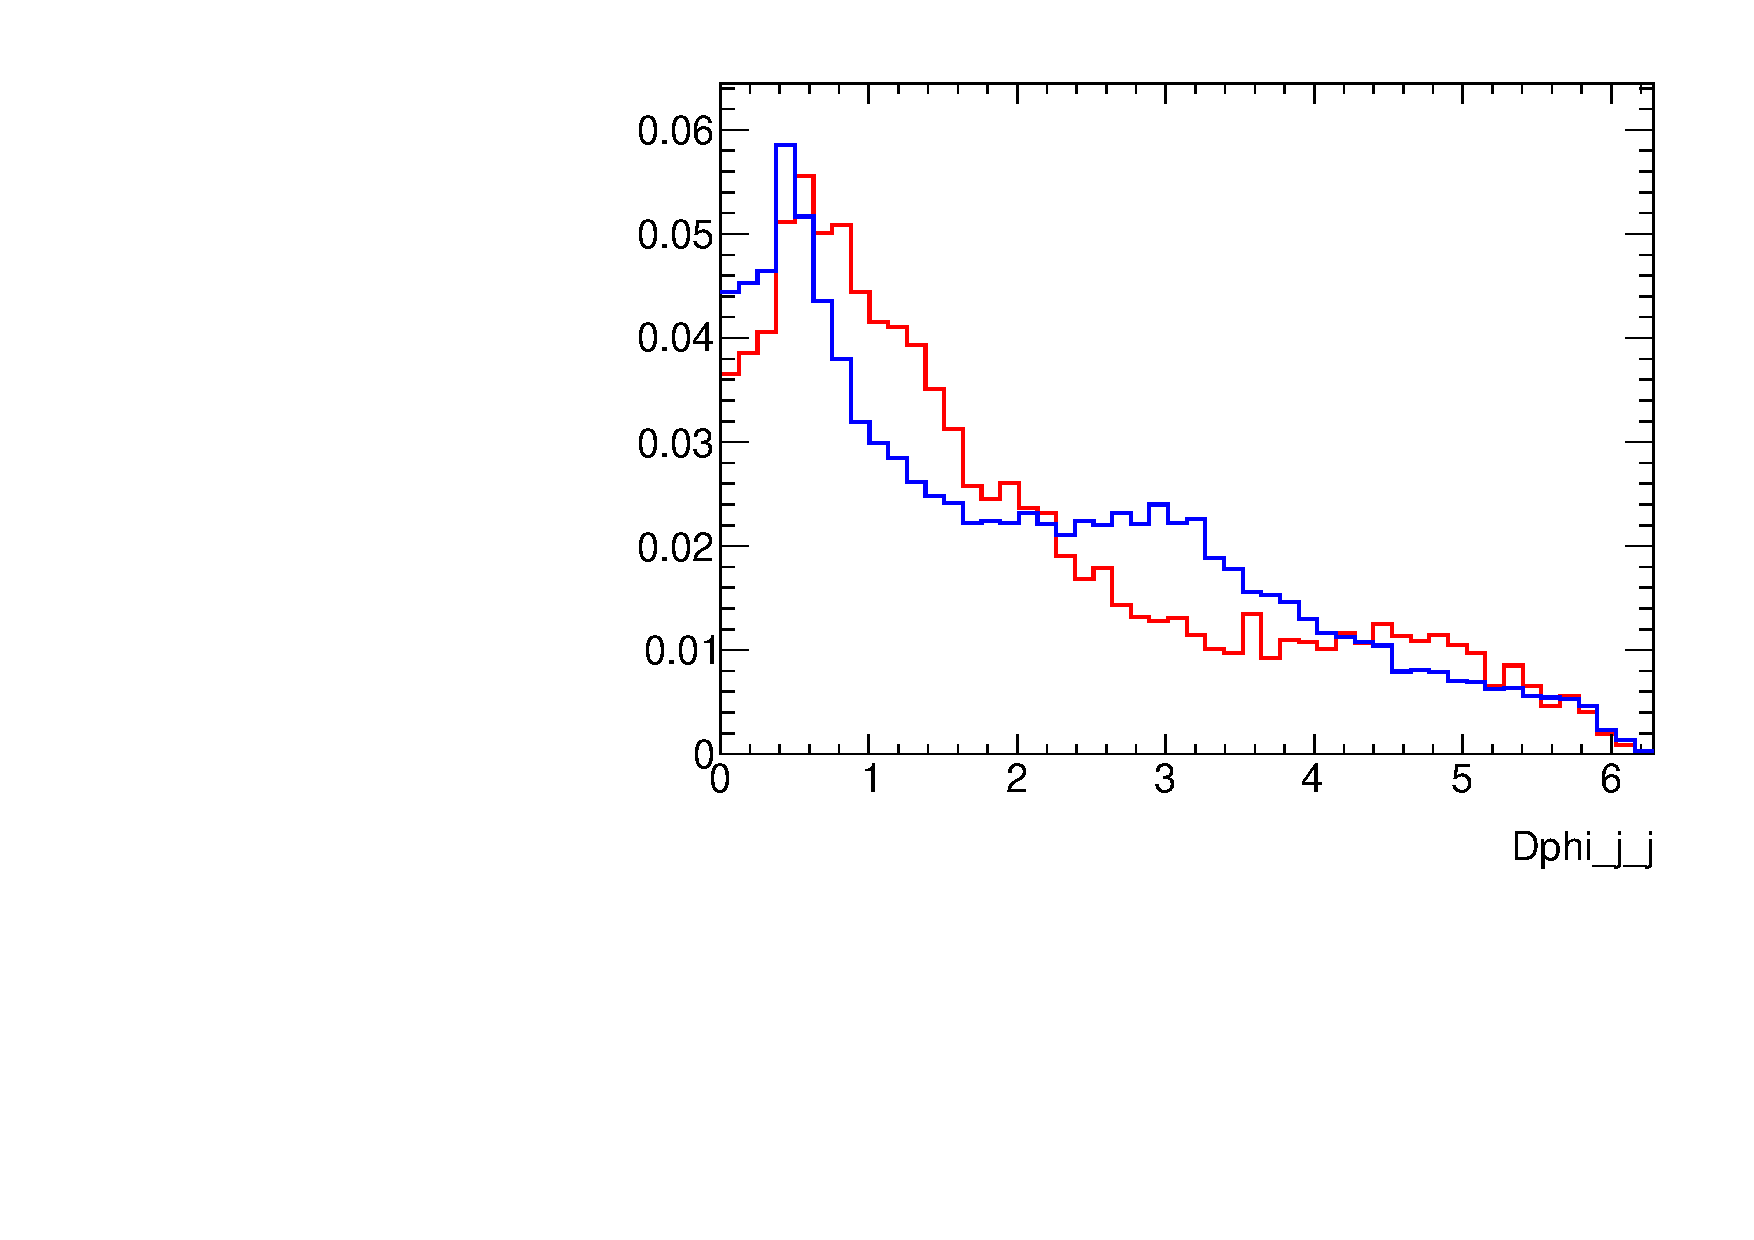
\includegraphics[width=.49\textwidth]{\resource{EWvQCD/Dphi_j_j.pdf}}
  \\
  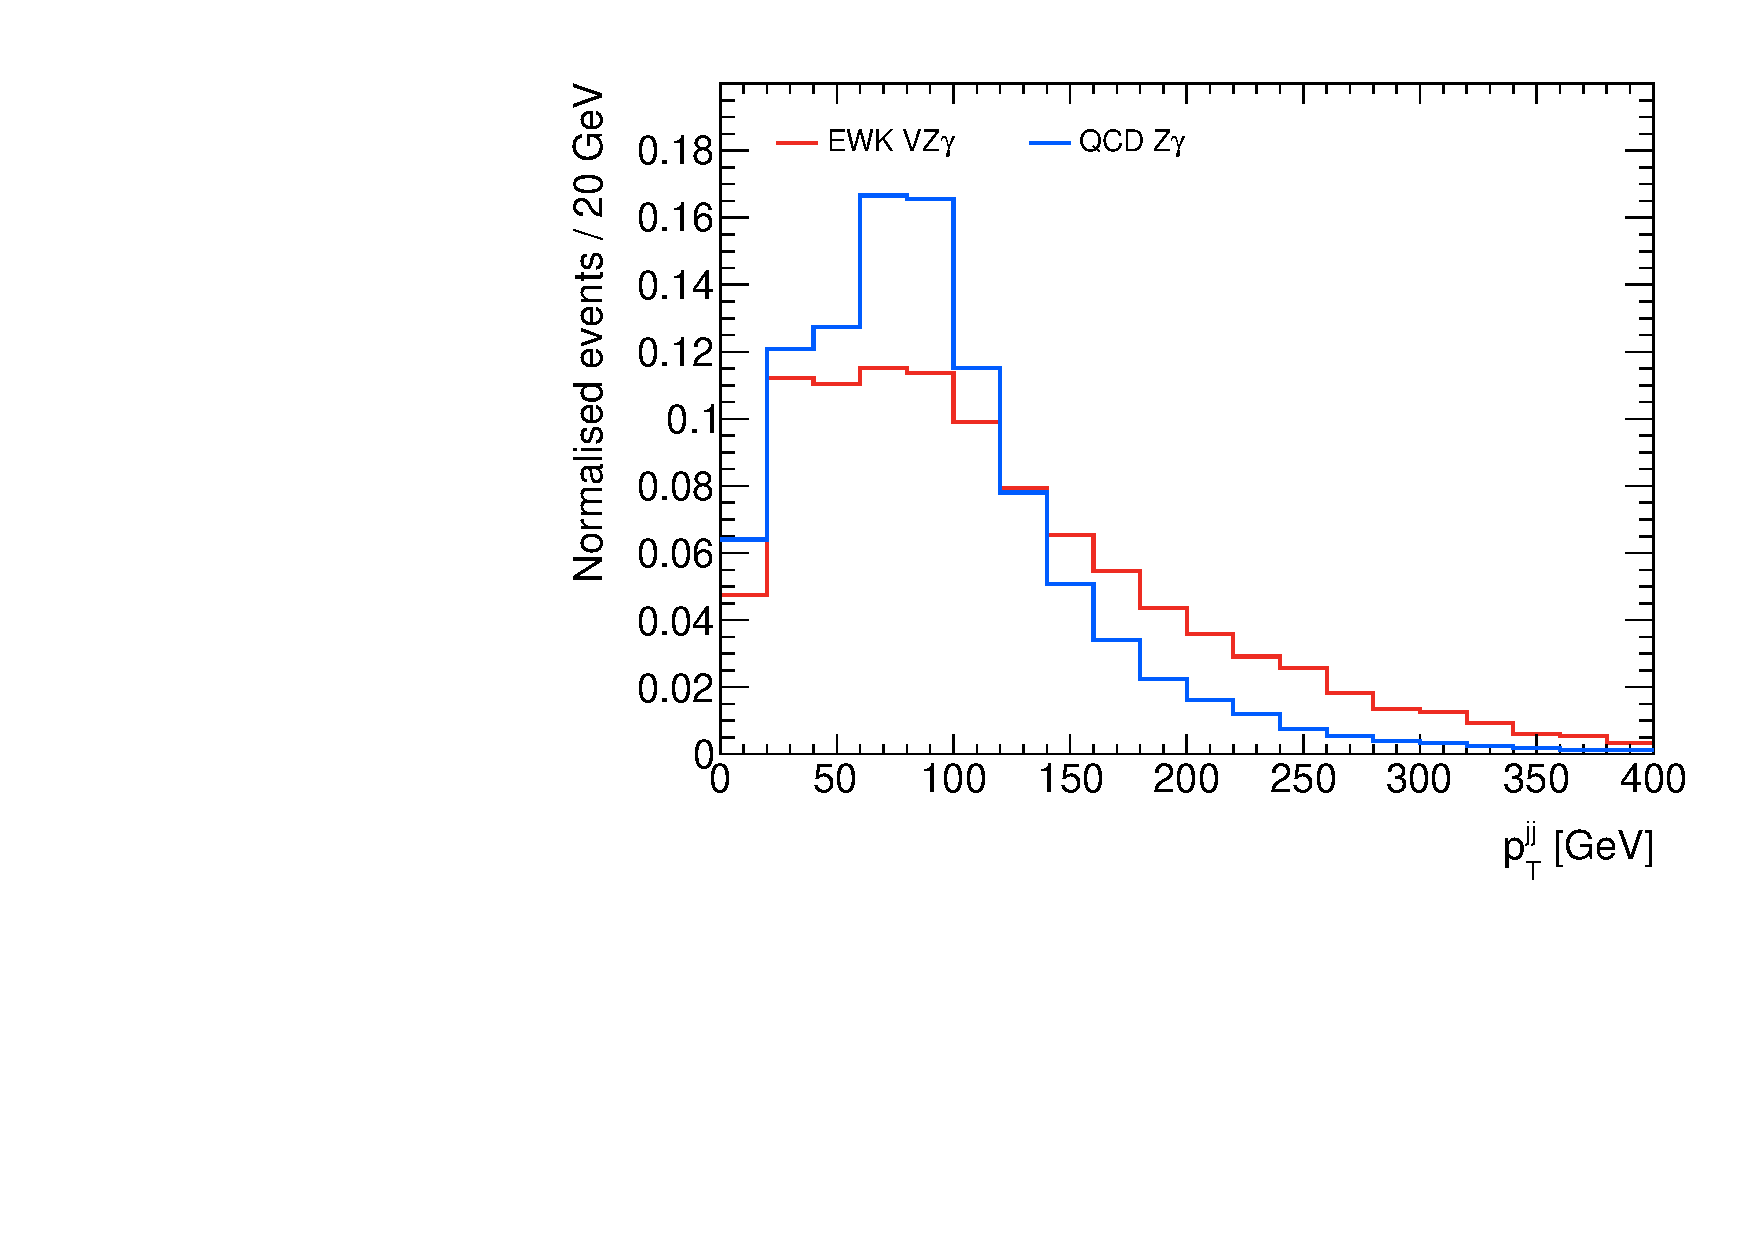
\includegraphics[width=.49\textwidth]{\resource{EWvQCD/pT_jj.pdf}}
  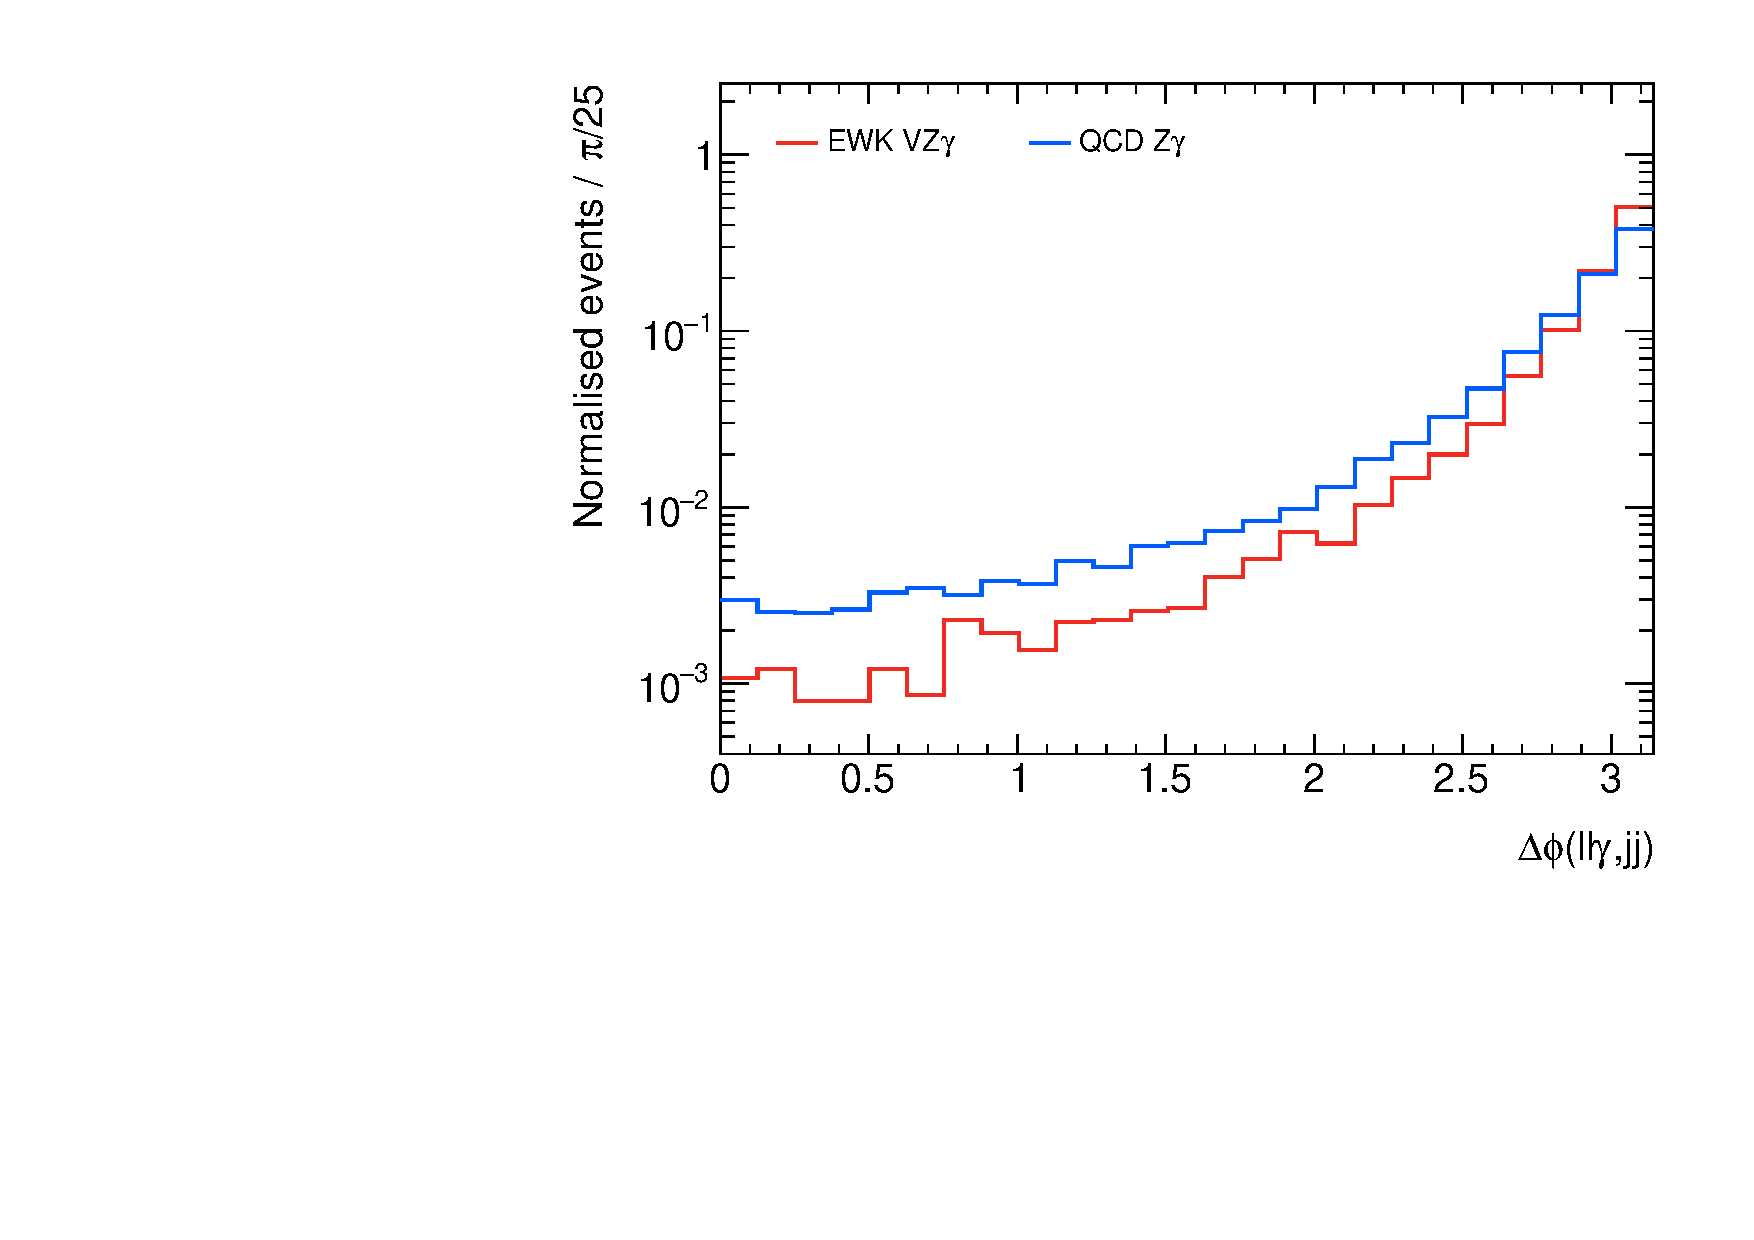
\includegraphics[width=.49\textwidth]{\resource{EWvQCD/Dphi_lly_jj.pdf}}
  %
  \caption{
    Kinematic distributions, comparing \acs{EW} V\Zy production (red) to \acs{QCD}
    \Zyjj production (blue). Generated from the corresponding \ac{MC} samples
    with V\Zy preselection applied.
  }
  \label{fig:vzy-bdt-ewvqcd}
\end{figure}

Building a cut-based selection with sensitivity to the signal is difficult, more
advanced methods might push the background rejection further. This section
explores two methods for defining a signal-sensitive phase space for the
analysis: a cut-based approach and a \ac{BDT}, a machine learning classifier
introduced in Section [BDT section in theory chapter]. %TODO

These initial investigations were performed before many details of the analysis
were established and so have a unique phase space, detailed below.

% Section giving samples and phase-space for this study
\subsection{Phase space for preliminary studies}

The studies presented in this section use events from the \ac{EW} \VZy sample
(as defined in Section \ref{sec:vzy-selection-vzy}) as the signal and from the
\ac{QCD} \Zy sample as the background. All events are subject to the
preselection in Table \ref{tab:vzy-bdt-preliminaryselection}.  These cuts select
\Zy events with an earlier version of the full \Zy selection presented in
Section \ref{sec:methods-selection}.  No cuts are placed on the jets at this
stage.  Isolation, identification, and overlap removal for all objects are the
same as discussed in Section \ref{sec:methods-selection}.

\begin{table}
  \centering
  \renewcommand\arraystretch{1.3}
  \begin{tabular}{p{6em}l}
    \hline\hline
    \multicolumn{2}{c}{Background rejection studies preselection} \\
    \hline
    Photon & $N_\gamma \geq 1$ \\
           & $|\eta_\gamma| < 2.37$ \\
           & (excludes $1.37 < |\eta_\gamma| < 1.52$) \\
           & $p_T^\gamma > 15$ GeV \\
    \hline
    Lepton & $N_l = 2$ (OSSF)\\
           & $|\eta_e| < 2.47$ \\
           & (excludes $1.37 < |\eta_e| < 1.52$) \\
           & $|\eta_\mu| < 2.5$ \\
           & $p_T^{l,1} > 30$ GeV \\
           & $p_T^{l,2} > 20$ GeV \\
    \hline
    Boson  & $m_{ll} > 40$ GeV \\
    \hline\hline
  \end{tabular}
  \caption{
    Selection for events used in background rejection studies for the \VZy
    triboson analysis. This is the same as the \Zy selection in Table
    \ref{tab:anacom-zy-selection} but with a looser photon $p_T$ cut and no
    \ac{FSR} cut.
  }
  \label{tab:anacom-zy-selection}
\end{table}


% Section describing cut-based selection optimisation
\subsection{Cut-based background rejection}
% See plots here, from old codebase
% /mnt/naf/code/VZy-prep/extract_VZy/build/signifscan_nomjj2_SR1.pdf

% Section describing BDT optimisation
\subsection{\acs{BDT} for background rejection}

% TODO write BDT section in theory
% sources:
%http://dx.doi.org/10.1016/j.nima.2004.12.018
%https://arxiv.org/abs/2206.09645

